
\documentclass[twocolumn]{aastex62}
%\documentclass[defaultstyle,11pt]{thesis}
%\documentclass[]{report}
%\documentclass[]{article}
%\usepackage{aastex_hack}
%\usepackage{deluxetable}
%\documentclass[preprint]{aastex}
%\documentclass{aa}

\newcommand{\titlerunning}[1]{\shorttitle{#1}}
\newcommand{\authorrunning}[1]{\shortauthors{#1}}

\newcommand*\inst[1]{\unskip\hbox{\@textsuperscript{\normalfont$#1$}}}

%\newcount\aa@nbinstitutes
%
%\newcounter{aa@institutecnt}

\newcommand*\institute[1]{
  \begingroup
    \let\and\relax
    \renewcommand*\inst[1]{}%
    \renewcommand*\thanks[1]{}%
    \renewcommand*\email[1]{}%
    %\let\@@protect\protect
    %\let\protect\@unexpandable@protect
    %\global\aa@nbinstitutes \z@
    %\expandafter\aa@cntinstitutes\aa@institute\and\aa@nil\and
    %\restore@protect
  \endgroup
  \newcommand{\institutions}{#1}
}%

\let\oldarcsec\arcsec
\renewcommand\arcsec{\oldarcsec\xspace}%

%\renewcommand{\abstract}[1]{
%\begin{abstract}
%    #1
%\end{abstract}
%}

%\renewcommand\ion[2]{#1$\;${%
%\ifx\@currsize\normalsize\small \else
%\ifx\@currsize\small\footnotesize \else
%\ifx\@currsize\footnotesize\scriptsize \else
%\ifx\@currsize\scriptsize\tiny \else
%\ifx\@currsize\large\normalsize \else
%\ifx\@currsize\Large\large
%\fi\fi\fi\fi\fi\fi
%\rmfamily\@Roman{#2}}\relax}% 
%
%\renewcommand{ion}[2]{#1}{#2}

\renewcommand{\ion}[2]{\textup{#1\,\textsc{\lowercase{#2}}}}

%\newcommand{\uchii}{\ensuremath{\mathrm{\ion{UCH}{2}}}\xspace}
%\newcommand{\UCHII}{\ensuremath{\mathrm{\ion{UCH}{2}}}\xspace}
%\newcommand{\hchii}{\ensuremath{\mathrm{\ion{HCH}{2}}}\xspace}
%\newcommand{\HCHII}{\ensuremath{\mathrm{\ion{HCH}{2}}}\xspace}
%\newcommand{\hii}  {\ensuremath{\mathrm{\ion{H}{2}}}\xspace}

%\input{aamacros.tex}

\pdfminorversion=4


%%%%%%%%%%%%%%%%%%%%%%%%%%%%%%%%%%%%%%%%%%%%%%%%%%%%%%%%%%%%%%%%
%%%%%%%%%%%  see documentation for information about  %%%%%%%%%%
%%%%%%%%%%%  the options (11pt, defaultstyle, etc.)   %%%%%%%%%%
%%%%%%%  http://www.colorado.edu/its/docs/latex/thesis/  %%%%%%%
%%%%%%%%%%%%%%%%%%%%%%%%%%%%%%%%%%%%%%%%%%%%%%%%%%%%%%%%%%%%%%%%
%		\documentclass[typewriterstyle]{thesis}
% 		\documentclass[modernstyle]{thesis}
% 		\documentclass[modernstyle,11pt]{thesis}
%	 	\documentclass[modernstyle,12pt]{thesis}

%%%%%%%%%%%%%%%%%%%%%%%%%%%%%%%%%%%%%%%%%%%%%%%%%%%%%%%%%%%%%%%%
%%%%%%%%%%%    load any packages which are needed    %%%%%%%%%%%
%%%%%%%%%%%%%%%%%%%%%%%%%%%%%%%%%%%%%%%%%%%%%%%%%%%%%%%%%%%%%%%%
\usepackage{latexsym}		% to get LASY symbols
\usepackage{graphicx}		% to insert PostScript figures
%\usepackage{deluxetable}
\usepackage{rotating}		% for sideways tables/figures
\usepackage{natbib}  % Requires natbib.sty, available from http://ads.harvard.edu/pubs/bibtex/astronat/
\usepackage{savesym}
%\usepackage{pdflscape}
\usepackage{amssymb}
\usepackage{amsmath}
\usepackage{morefloats}
%\savesymbol{singlespace}
\savesymbol{doublespace}
%\usepackage{wrapfig}
%\usepackage{setspace}
\usepackage{xspace}
\usepackage{color}
%\usepackage{multicol}
\usepackage{mdframed}
\usepackage{url}
\usepackage{subfigure}
%\usepackage{emulateapj}
%\usepackage{lscape}
\usepackage{grffile}
\usepackage{import}
\usepackage[utf8]{inputenc}
%\usepackage{longtable}
\usepackage{booktabs}
%\usepackage[yyyymmdd,hhmmss]{datetime}
\usepackage{fancyhdr}
%\usepackage[colorlinks=true,citecolor=blue,linkcolor=cyan]{hyperref}

\usepackage[hang,flushmargin]{footmisc}
\usepackage{ifpdf}


%\usepackage{standalone}
%\standalonetrue






\newcommand{\paa}{Pa\ensuremath{\alpha}}
\newcommand{\brg}{Br\ensuremath{\gamma}}
\newcommand{\msun}{\ensuremath{M_{\odot}}\xspace}			%  Msun
\newcommand{\mdot}{\ensuremath{\dot{M}}\xspace}
\newcommand{\lsun}{\ensuremath{L_{\odot}}\xspace}			%  Lsun
\newcommand{\rsun}{\ensuremath{R_{\odot}}\xspace}			%  Rsun
\newcommand{\lbol}{\ensuremath{L_{\mathrm{bol}}\xspace}}	%  Lbol
\newcommand{\ks}{K\ensuremath{_{\mathrm{s}}}}		%  Ks
\newcommand{\hh}{\ensuremath{\textrm{H}_{2}}\xspace}			%  H2
\newcommand{\dens}{\ensuremath{n(\hh) [\percc]}\xspace}
\newcommand{\formaldehyde}{\ensuremath{\textrm{H}_2\textrm{CO}}\xspace}
\newcommand{\formamide}{\ensuremath{\textrm{NH}_2\textrm{CHO}}\xspace}
\newcommand{\formaldehydeIso}{\ensuremath{\textrm{H}_2~^{13}\textrm{CO}}\xspace}
\newcommand{\methanol}{\ensuremath{\textrm{CH}_3\textrm{OH}}\xspace}
\newcommand{\ortho}{\ensuremath{\textrm{o-H}_2\textrm{CO}}\xspace}
\newcommand{\para}{\ensuremath{\textrm{p-H}_2\textrm{CO}}\xspace}
\newcommand{\oneone}{\ensuremath{1_{1,0}-1_{1,1}}\xspace}
\newcommand{\twotwo}{\ensuremath{2_{1,1}-2_{1,2}}\xspace}
\newcommand{\threethree}{\ensuremath{3_{1,2}-3_{1,3}}\xspace}
\newcommand{\threeohthree}{\ensuremath{3_{0,3}-2_{0,2}}\xspace}
\newcommand{\threetwotwo}{\ensuremath{3_{2,2}-2_{2,1}}\xspace}
\newcommand{\threetwoone}{\ensuremath{3_{2,1}-2_{2,0}}\xspace}
\newcommand{\fourtwotwo}{\ensuremath{4_{2,2}-3_{1,2}}\xspace} % CH3OH 218.4 GHz
\newcommand{\methylcyanide}{\ensuremath{\textrm{CH}_{3}\textrm{CN}}\xspace}
\newcommand{\ketene}{\ensuremath{\textrm{H}_{2}\textrm{CCO}}\xspace}
\newcommand{\ethylcyanide}{\ensuremath{\textrm{CH}_3\textrm{CH}_2\textrm{CN}}\xspace}
\newcommand{\cyanoacetylene}{\ensuremath{\textrm{HC}_{3}\textrm{N}}\xspace}
\newcommand{\methylformate}{\ensuremath{\textrm{CH}_{3}\textrm{OCHO}}\xspace}
\newcommand{\dimethylether}{\ensuremath{\textrm{CH}_{3}\textrm{OCH}_{3}}\xspace}
\newcommand{\gaucheethanol}{\ensuremath{\textrm{g-CH}_3\textrm{CH}_2\textrm{OH}}\xspace}
\newcommand{\acetone}{\ensuremath{\left[\textrm{CH}_{3}\right]_2\textrm{CO}}\xspace}
\newcommand{\methyleneamidogen}{\ensuremath{\textrm{H}_{2}\textrm{CN}}\xspace}
\newcommand{\Rone}{\ensuremath{\para~S_{\nu}(\threetwoone) / S_{\nu}(\threeohthree)}\xspace}
\newcommand{\Rtwo}{\ensuremath{\para~S_{\nu}(\threetwotwo) / S_{\nu}(\threetwoone)}\xspace}
\newcommand{\JKaKc}{\ensuremath{J_{K_a K_c}}}
\newcommand{\water}{H$_{2}$O\xspace}		%  H2O
\newcommand{\feii}{\ion{Fe}{ii}\xspace}		%  FeII

\newcommand{\uchii}{\ion{UCH}{ii}\xspace}
\newcommand{\UCHII}{\ion{UCH}{ii}\xspace}
\newcommand{\hchii}{\ion{HCH}{ii}\xspace}
\newcommand{\HCHII}{\ion{HCH}{ii}\xspace}
\newcommand{\hii}{\ion{H}{ii}\xspace}

\newcommand{\hi}{H~{\sc i}\xspace}
\newcommand{\Hii}{\hii}
\newcommand{\HII}{\hii}
\newcommand{\Xform}{\ensuremath{X_{\formaldehyde}}}
\newcommand{\kms}{\textrm{km~s}\ensuremath{^{-1}}\xspace}	%  km s-1
\newcommand{\nsample}{456\xspace}
\newcommand{\CFR}{5\xspace} % nMPC / 0.25 / 2 (6 for W51 once, 8 for W51 twice) REFEDIT: With f_observed=0.3, becomes 3/2./0.3 = 5
\newcommand{\permyr}{\ensuremath{\mathrm{Myr}^{-1}}\xspace}
\newcommand{\pers}{\ensuremath{\mathrm{s}^{-1}}\xspace}
\newcommand{\perspc}{\ensuremath{\mathrm{pc}^{-2}}\xspace}
\newcommand{\tsuplim}{0.5\xspace} % upper limit on starless timescale
\newcommand{\ncandidates}{18\xspace}
\newcommand{\mindist}{8.7\xspace}
\newcommand{\rcluster}{2.5\xspace}
\newcommand{\ncomplete}{13\xspace}
\newcommand{\middistcut}{13.0\xspace}
\newcommand{\nMPC}{3\xspace} % only count W51 once.  W51, W49, G010
\newcommand{\obsfrac}{30}
\newcommand{\nMPCtot}{10\xspace} % = nmpc / obsfrac
\newcommand{\nMPCtoterr}{6\xspace} % = sqrt(nmpc) / obsfrac
\newcommand{\plaw}{2.1\xspace}
\newcommand{\plawerr}{0.3\xspace}
\newcommand{\mmin}{\ensuremath{10^4~\msun}\xspace}
%\newcommand{\perkmspc}{\textrm{per~km~s}\ensuremath{^{-1}}\textrm{pc}\ensuremath{^{-1}}\xspace}	%  km s-1 pc-1
\newcommand{\kmspc}{\textrm{km~s}\ensuremath{^{-1}}\textrm{pc}\ensuremath{^{-1}}\xspace}	%  km s-1 pc-1
\newcommand{\sqcm}{cm$^{2}$\xspace}		%  cm^2
\newcommand{\percc}{\ensuremath{\textrm{cm}^{-3}}\xspace}
\newcommand{\perpc}{\ensuremath{\textrm{pc}^{-1}}\xspace}
\newcommand{\persc}{\ensuremath{\textrm{cm}^{-2}}\xspace}
\newcommand{\persr}{\ensuremath{\textrm{sr}^{-1}}\xspace}
\newcommand{\peryr}{\ensuremath{\textrm{yr}^{-1}}\xspace}
\newcommand{\perkmspc}{\textrm{km~s}\ensuremath{^{-1}}\textrm{pc}\ensuremath{^{-1}}\xspace}	%  km s-1 pc-1
\newcommand{\perkms}{\textrm{per~km~s}\ensuremath{^{-1}}\xspace}	%  km s-1 
\newcommand{\um}{\ensuremath{\mu \textrm{m}}\xspace}    % micron
\newcommand{\microjy}{\ensuremath{\mu\textrm{Jy}}\xspace}    % micron
\newcommand{\microJy}{\ensuremath{\mu\textrm{Jy}}\xspace}    % micron
\newcommand{\mum}{\um}
\newcommand{\htwo}{\ensuremath{\textrm{H}_2}}
\newcommand{\Htwo}{\ensuremath{\textrm{H}_2}}
\newcommand{\HtwoO}{\ensuremath{\textrm{H}_2\textrm{O}}}
\newcommand{\htwoo}{\ensuremath{\textrm{H}_2\textrm{O}}}
\newcommand{\ha}{\ensuremath{\textrm{H}\alpha}}
\newcommand{\hb}{\ensuremath{\textrm{H}\beta}}
\newcommand{\so}{SO~\ensuremath{5_6-4_5}\xspace}
\newcommand{\SO}{SO~\ensuremath{1_2-1_1}\xspace}
\newcommand{\ammonia}{NH\ensuremath{_3}\xspace}
\newcommand{\twelveco}{\ensuremath{^{12}\textrm{CO}}\xspace}
\newcommand{\thirteenco}{\ensuremath{^{13}\textrm{CO}}\xspace}
\newcommand{\ceighteeno}{\ensuremath{\textrm{C}^{18}\textrm{O}}\xspace}
\def\ee#1{\ensuremath{\times10^{#1}}}
\newcommand{\degrees}{\ensuremath{^{\circ}}}
% can't have \degree because I'm getting a degree...
\newcommand{\lowirac}{800}
\newcommand{\highirac}{8000}
\newcommand{\lowmips}{600}
\newcommand{\highmips}{5000}
\newcommand{\perbeam}{\ensuremath{\textrm{beam}^{-1}}\xspace}
\newcommand{\ds}{\ensuremath{\textrm{d}s}}
\newcommand{\dnu}{\ensuremath{\textrm{d}\nu}}
\newcommand{\dv}{\ensuremath{\textrm{d}v}}
\def\secref#1{Section \ref{#1}}
\def\eqref#1{Equation \ref{#1}}
\def\facility#1{#1}
%\newcommand{\arcmin}{'}

\newcommand{\necluster}{Sh~2-233IR~NE}
\newcommand{\swcluster}{Sh~2-233IR~SW}
\newcommand{\region}{IRAS 05358}

\newcommand{\nwfive}{40}
\newcommand{\nouter}{15}

\newcommand{\vone}{{\rm v}1.0\xspace}
\newcommand{\vtwo}{{\rm v}2.0\xspace}
\newcommand\mjysr{\ensuremath{{\rm MJy~sr}^{-1}}}
\newcommand\jybm{\ensuremath{{\rm Jy~bm}^{-1}}}
\newcommand\nbolocat{8552\xspace}
\newcommand\nbolocatnew{548\xspace}
\newcommand\nbolocatnonew{8004\xspace} % = nbolocat-nbolocatnew
%\renewcommand\arcdeg{\mbox{$^\circ$}\xspace} 
%\renewcommand\arcmin{\mbox{$^\prime$}\xspace} 
%\renewcommand\arcsec{\mbox{$^{\prime\prime}$}\xspace} 

\newcommand{\todo}[1]{\textcolor{red}{#1}}
\newcommand{\okinfinal}[1]{{#1}}
%% only needed if not aastex
%\newcommand{\keywords}[1]{}
%\newcommand{\email}[1]{}
%\newcommand{\affil}[1]{}


%aastex hack
%\newcommand\arcdeg{\mbox{$^\circ$}}%
%\newcommand\arcmin{\mbox{$^\prime$}\xspace}%
%\newcommand\arcsec{\mbox{$^{\prime\prime}$}\xspace}%

%\newcommand\epsscale[1]{\gdef\eps@scaling{#1}}
%
%\newcommand\plotone[1]{%
% \typeout{Plotone included the file #1}
% \centering
% \leavevmode
% \includegraphics[width={\eps@scaling\columnwidth}]{#1}%
%}%
%\newcommand\plottwo[2]{{%
% \typeout{Plottwo included the files #1 #2}
% \centering
% \leavevmode
% \columnwidth=.45\columnwidth
% \includegraphics[width={\eps@scaling\columnwidth}]{#1}%
% \hfil
% \includegraphics[width={\eps@scaling\columnwidth}]{#2}%
%}}%


%\newcommand\farcm{\mbox{$.\mkern-4mu^\prime$}}%
%\let\farcm\farcm
%\newcommand\farcs{\mbox{$.\!\!^{\prime\prime}$}}%
%\let\farcs\farcs
%\newcommand\fp{\mbox{$.\!\!^{\scriptscriptstyle\mathrm p}$}}%
%\newcommand\micron{\mbox{$\mu$m}}%
%\def\farcm{%
% \mbox{.\kern -0.7ex\raisebox{.9ex}{\scriptsize$\prime$}}%
%}%
%\def\farcs{%
% \mbox{%
%  \kern  0.13ex.%
%  \kern -0.95ex\raisebox{.9ex}{\scriptsize$\prime\prime$}%
%  \kern -0.1ex%
% }%
%}%

\def\Figure#1#2#3#4#5{
\begin{figure*}[!htp]
\includegraphics[scale=#4,width=#5]{#1}
\caption{#2}
\label{#3}
\end{figure*}
}

\def\FigureOneCol#1#2#3#4#5{
\begin{figure}[!htp]
\includegraphics[scale=#4,width=#5]{#1}
\caption{#2}
\label{#3}
\end{figure}
}


\def\WrapFigure#1#2#3#4#5#6{
\begin{wrapfigure}{#6}{0.5\textwidth}
\includegraphics[scale=#4,width=#5]{#1}
\caption{#2}
\label{#3}
\end{wrapfigure}
}

% % #1 - filename
% % #2 - caption
% % #3 - label
% % #4 - epsscale
% % #5 - R or L?
% \def\WrapFigure#1#2#3#4#5#6{
% \begin{wrapfigure}[#6]{#5}{0.45\textwidth}
% %  \centercaption
% %  \vspace{-14pt}
%   \epsscale{#4}
%   \includegraphics[scale=#4]{#1}
%   \caption{#2}
%   \label{#3}
% \end{wrapfigure}
% }

\def\RotFigure#1#2#3#4#5{
\begin{sidewaysfigure*}[!htp]
\includegraphics[scale=#4,width=#5]{#1}
\caption{#2}
\label{#3}
\end{sidewaysfigure*}
}

\def\FigureSVG#1#2#3#4{
\begin{figure*}[!htp]
    \def\svgwidth{#4}
    \input{#1}
    \caption{#2}
    \label{#3}
\end{figure*}
}

% originally intended to be included in a two-column paper
% this is in includegraphics: ,width=3in
% but, not for thesis
\def\OneColFigure#1#2#3#4#5{
\begin{figure}[!htpb]
\epsscale{#4}
\includegraphics[scale=#4,angle=#5]{#1}
\caption{#2}
\label{#3}
\end{figure}
}

\def\SubFigure#1#2#3#4#5{
\begin{figure*}[!htp]
\addtocounter{figure}{-1}
\epsscale{#4}
\includegraphics[angle=#5]{#1}
\caption{#2}
\label{#3}
\end{figure*}
}


\def\FigureTwo#1#2#3#4#5#6{
\begin{figure*}[!htp]
\subfigure[]{ \includegraphics[scale=#5,width=#6]{#1} }
\subfigure[]{ \includegraphics[scale=#5,width=#6]{#2} }
\caption{#3}
\label{#4}
\end{figure*}
}

\def\FigureTwoAA#1#2#3#4#5#6{
\begin{figure*}[!htp]
\subfigure[]{ \includegraphics[scale=#5,width=#6]{#1} }
\subfigure[]{ \includegraphics[scale=#5,width=#6]{#2} }
\caption{#3}
\label{#4}
\end{figure*}
}

\newenvironment{rotatepage}
{}{}


\def\RotFigureTwoAA#1#2#3#4#5#6{
\begin{rotatepage}
\begin{sidewaysfigure*}[!htp]
\subfigure[]{ \includegraphics[scale=#5,width=#6]{#1} }
\\
\subfigure[]{ \includegraphics[scale=#5,width=#6]{#2} }
\caption{#3}
\label{#4}
\end{sidewaysfigure*}
\end{rotatepage}
}

\def\RotFigureThree#1#2#3#4#5#6#7{
\begin{rotatepage}
\begin{sidewaysfigure*}[!htp]
\subfigure[]{ \includegraphics[scale=#6,width=#7]{#1} }
\\
\subfigure[]{ \includegraphics[scale=#6,width=#7]{#2} }
\\
\subfigure[]{ \includegraphics[scale=#6,width=#7]{#3} }
\caption{#4}
\label{#5}
\end{sidewaysfigure*}
\end{rotatepage}
\clearpage
}

\def\FigureThree#1#2#3#4#5#6#7{
\begin{figure*}[!htp]
\subfigure[]{ \includegraphics[scale=#6,width=#7]{#1} }
\subfigure[]{ \includegraphics[scale=#6,width=#7]{#2} }
\subfigure[]{ \includegraphics[scale=#6,width=#7]{#3} }
\caption{#4}
\label{#5}
\end{figure*}
}



\def\SubFigureTwo#1#2#3#4#5{
\begin{figure*}[!htp]
\addtocounter{figure}{-1}
\epsscale{#5}
\plottwo{#1}{#2}
\caption{#3}
\label{#4}
\end{figure*}
}

\def\FigureFour#1#2#3#4#5#6#7#8{
\begin{figure*}[!htp]
\subfigure[]{ \includegraphics[scale=#7,width=#8]{#1} }
\subfigure[]{ \includegraphics[scale=#7,width=#8]{#2} }
\subfigure[]{ \includegraphics[scale=#7,width=#8]{#3} }
\subfigure[]{ \includegraphics[scale=#7,width=#8]{#4} }
\caption{#5}
\label{#6}
\end{figure*}
}

\def\FigureFourVertical#1#2#3#4#5#6#7#8{
\begin{figure*}[!htp]
\subfigure[]{ \includegraphics[scale=#7,width=#8]{#1} }
\vspace{0.001mm} \\
\subfigure[]{ \includegraphics[scale=#7,width=#8]{#2} }
\vspace{0.001mm} \\
\subfigure[]{ \includegraphics[scale=#7,width=#8]{#3} }
\vspace{0.001mm} \\
\subfigure[]{ \includegraphics[scale=#7,width=#8]{#4} }
\vspace{0.001mm}
\caption{#5}
\label{#6}
\end{figure*}
}

\def\FigureFourPDF#1#2#3#4#5#6{
\begin{figure*}[!htp]
\subfigure[]{ \includegraphics[width=3in,type=pdf,ext=.pdf,read=.pdf]{#1} }
\subfigure[]{ \includegraphics[width=3in,type=pdf,ext=.pdf,read=.pdf]{#2} }
\subfigure[]{ \includegraphics[width=3in,type=pdf,ext=.pdf,read=.pdf]{#3} }
\subfigure[]{ \includegraphics[width=3in,type=pdf,ext=.pdf,read=.pdf]{#4} }
\caption{#5}
\label{#6}
\end{figure*}
}

\def\FigureThreePDF#1#2#3#4#5{
\begin{figure*}[!htp]
\subfigure[]{ \includegraphics[width=3in,type=pdf,ext=.pdf,read=.pdf]{#1} }
\subfigure[]{ \includegraphics[width=3in,type=pdf,ext=.pdf,read=.pdf]{#2} }
\subfigure[]{ \includegraphics[width=3in,type=pdf,ext=.pdf,read=.pdf]{#3} }
\caption{#4}
\label{#5}
\end{figure*}
}

\def\Table#1#2#3#4#5{
%\renewcommand{\thefootnote}{\alph{footnote}}
\begin{table}
\caption{#2}
\label{#3}
    \begin{tabular}{#1}
        \hline\hline
        #4
        \hline
        #5
        \hline
    \end{tabular}
\end{table}
%\renewcommand{\thefootnote}{\arabic{footnote}}
}


%\def\Table#1#2#3#4#5#6{
%%\renewcommand{\thefootnote}{\alph{footnote}}
%\begin{deluxetable}{#1}
%\tablewidth{0pt}
%\tabletypesize{\footnotesize}
%\tablecaption{#2}
%\tablehead{#3}
%\startdata
%\label{#4}
%#5
%\enddata
%\bigskip
%#6
%\end{deluxetable}
%%\renewcommand{\thefootnote}{\arabic{footnote}}
%}

%\def\tablenotetext#1#2{
%\footnotetext[#1]{#2}
%}

% \def\LongTable#1#2#3#4#5#6#7#8{
% % required to get tablenotemark to work: http://www2.astro.psu.edu/users/stark/research/psuthesis/longtable.html
% \renewcommand{\thefootnote}{\alph{footnote}}
% \begin{longtable}{#1}
% \caption[#2]{#2}
% \label{#4} \\
% 
%  \\
% \hline 
% #3 \\
% \hline
% \endfirsthead
% 
% \hline
% #3 \\
% \hline
% \endhead
% 
% \hline
% \multicolumn{#8}{r}{{Continued on next page}} \\
% \hline
% \endfoot
% 
% \hline 
% \endlastfoot
% #7 \\
% 
% #5
% \hline
% #6 \\
% 
% \end{longtable}
% \renewcommand{\thefootnote}{\arabic{footnote}}
% }

\def\TallFigureTwo#1#2#3#4#5#6{
\begin{figure*}[htp]
\epsscale{#5}
\subfigure[]{ \includegraphics[width=#6]{#1} }
\subfigure[]{ \includegraphics[width=#6]{#2} }
\caption{#3}
\label{#4}
\end{figure*}
}

		% file containing author's macro definitions
%%% This file is generated by the Makefile.
\newcommand{\githash}{008e348}\newcommand{\gitdate}{2018-10-19\xspace}\newcommand{\gitauthor}{Adam Ginsburg (keflavich)\xspace}

\newcommand{\sourcei}{SrcI\xspace}
\newcommand{\sourcen}{SrcN\xspace}
\newcommand{\sourcex}{SrcX\xspace}
\begin{document}
\newcommand{\nraojansky}{\affiliation{\it{Jansky fellow of the National Radio Astronomy Observatory, 1003 Lopezville Rd, Socorro, NM 87801 USA }}}
\newcommand{\nrao}{\affiliation{\it{National Radio Astronomy Observatory, 1003 Lopezville Rd, Socorro, NM 87801 USA }}}
\newcommand{\nraocv}{\affiliation{\it{National Radio Astronomy Observatory, Charlottesville, VA 22903 USA }}}
\newcommand{\cfa}{\affiliation{\it{Harvard-Smithsonian Center for Astrophysics, Cambridge, MA 02138 USA }}}
\newcommand{\hubble}{\altaffiliation{B.A.M. is a Hubble Fellow of the National Radio Astronomy\\ Observatory.}}


\newcommand{\radboud}{\affiliation{\it{Department of Astrophysics/IMAPP, Radboud University Nijmegen, PO Box 9010, 6500 GL Nijmegen, the Netherlands}}}
\newcommand{\allegro}{\affiliation{\it{ALLEGRO/Leiden Observatory, Leiden University, PO Box 9513, 2300 RA Leiden, the Netherlands}}}
\newcommand{\casa}{\affiliation{\it{CASA, University of Colorado, 389-UCB, Boulder, CO 80309}} }

\newcommand{\berkeley}{\affiliation{\it{Radio Astronomy Laboratory, University of California, Berkeley, CA 94720}} }

\author[0000-0001-6431-9633]{Adam Ginsburg}
\nraojansky
%\eso

%\author{
%Adam Ginsburg{\nrao},
%\begin{flushleft}
%\institutions
%\end{flushleft}
%        }
%
%\institute{
%    {\nrao}{\it{National Radio Astronomy Observatory, Socorro, NM 87801 USA\\
%                      \email{aginsbur@nrao.edu} 
%                      }} \\
%    }
%
\correspondingauthor{Adam Ginsburg}
\email{aginsbur@nrao.edu; adam.g.ginsburg@gmail.com}

\author{Brett McGuire}
\hubble
\nraocv
\cfa

\author{Richard Plambeck}
\berkeley

\author{John Bally}
\casa

\author{Ciriaco Goddi}
\allegro
\radboud


\author{Melvyn Wright}
\berkeley


\title{Orion \sourcei's disk is salty}
\begin{abstract}
    We report the detection of NaCl and KCl and the $^{37}$Cl and $^{41}$K
    isotopologues toward the disk around Orion \sourcei.
    This is the first detection of these molecules in the interstellar
    medium not associated with the ejecta of evolved stars.
    These lines are likely to be unique tracers of a rare process, either
    the birth of high-mass stars or the aftermath of a stellar collision.
\end{abstract}

\section{Introduction}
Molecules consisting of alkali metals and halogens have been detected
toward evolved stars including IRC +10216 \citep{Cernicharo1987a}, 


\section{Observations}
The observations presented here are described in \citet{Ginsburg2018a} as part
of ALMA project 2016.1.00165.S.  We use the robust 0.5 weighted spectral cubes
from all three bands (B3 3 mm, B6 1 mm, B7 0.85 mm) for the spectral analysis
presented here.

Appendix D of that paper describes the spectral extraction method,
which we summarize here.  We used the U232.511 line (which we identify here as
NaCl v=1 J=18-17) to create a velocity centroid map.  For each spectrum with
a measured velocity, we shifted the spectrum to 0 \kms, then averaged those
spectra.  The averaging area is approximately the extent of the continuum
disk, 0.03 square arcseconds, or about 20 beam areas at band 6.

In that appendix, we reported that ``there is no consistent pattern to the
detected lines and no individual species can explain more than a few of the
observed lines.''  This statement was incorrect, as there are obvious carriers
for the majority of the unidentified lines that we had simply overlooked:
NaCl (11 transitions in-band, 10 detections), Na$^{37}$Cl (8 transitions, 8
detections), KCl (8 transitions, 8 detections), $^{41}$KCl (8 transitions, 4
detections), and K$^{37}$Cl (7 transitions, 5 detections).
The nondetections all occur in the wings of other lines or in absorption
features from the surrounding molecular cloud.

Figures 1-3 shows the spectra with all lines labeled.

\begin{figure*}[!htp]
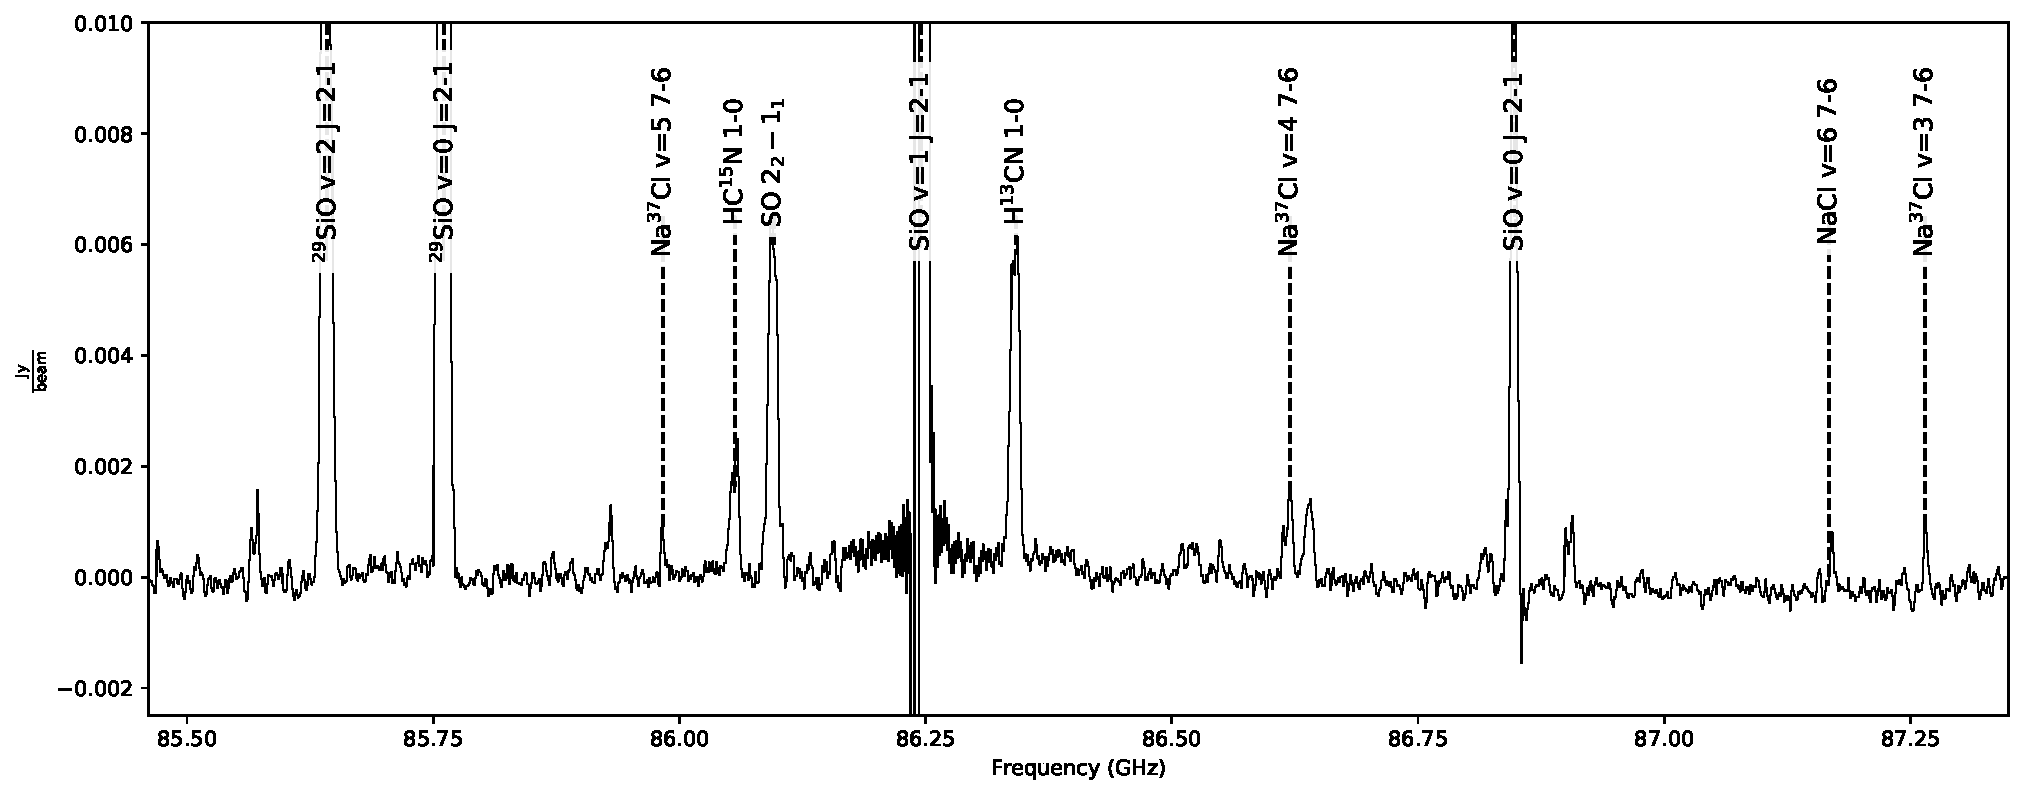
\includegraphics[scale=1,width=6in]{figures/lines_labeled_OrionSourceI_B3_spw0_robust0.5.pdf}
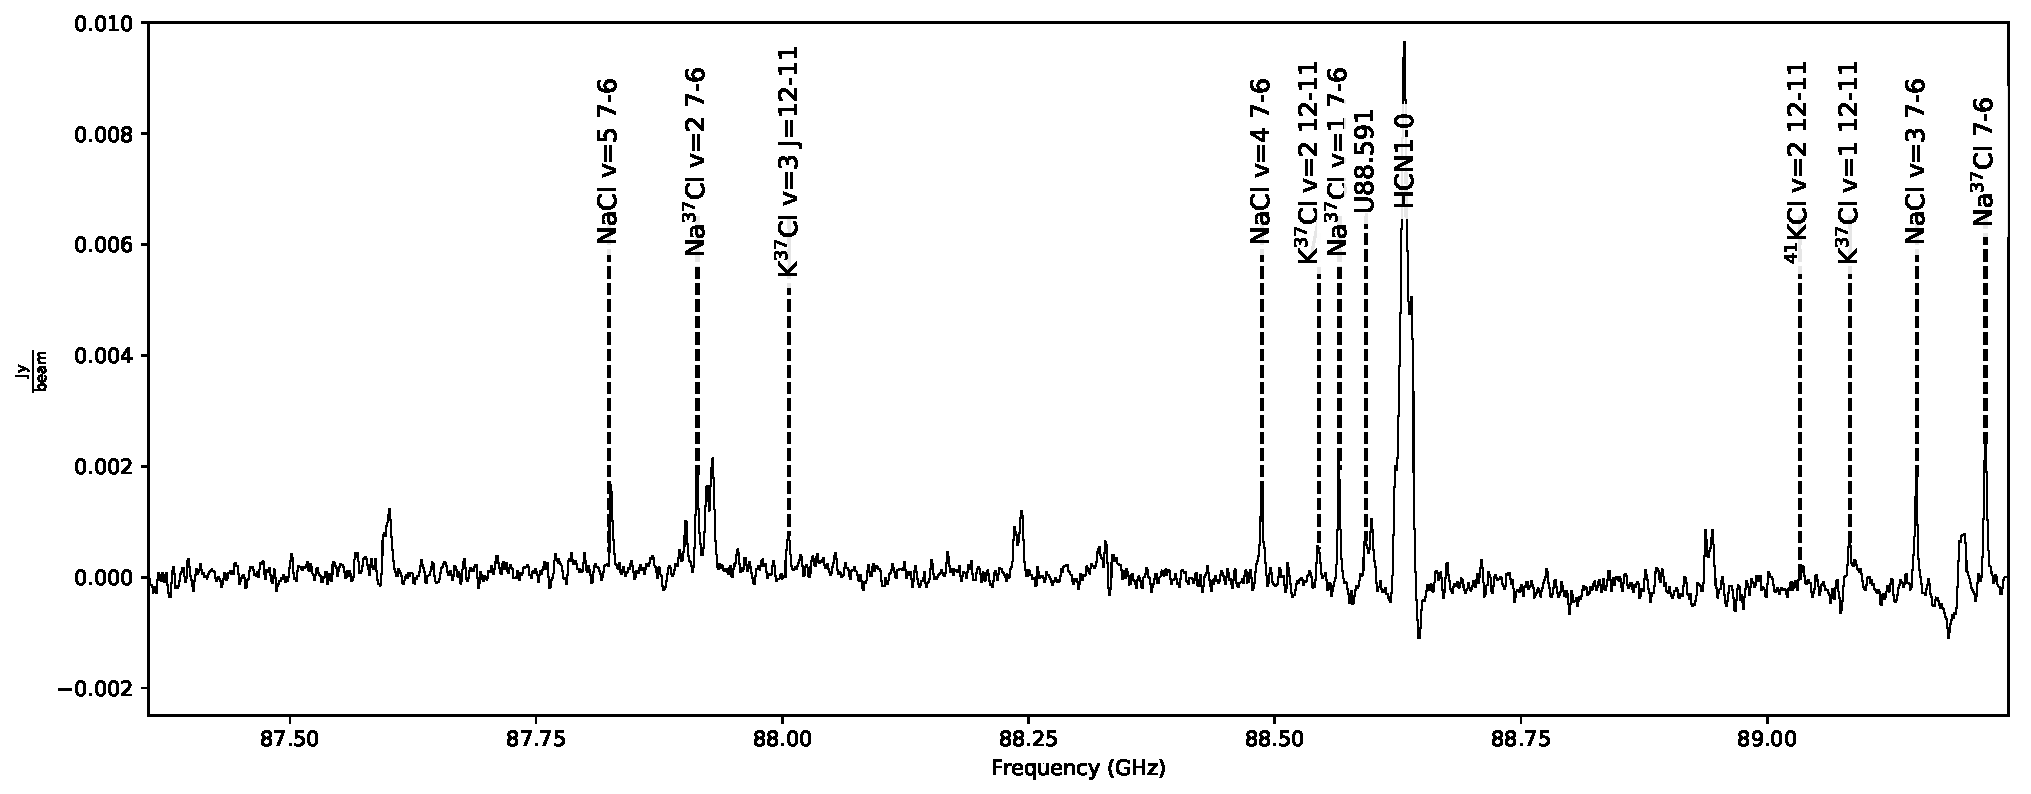
\includegraphics[scale=1,width=6in]{figures/lines_labeled_OrionSourceI_B3_spw1_robust0.5.pdf}
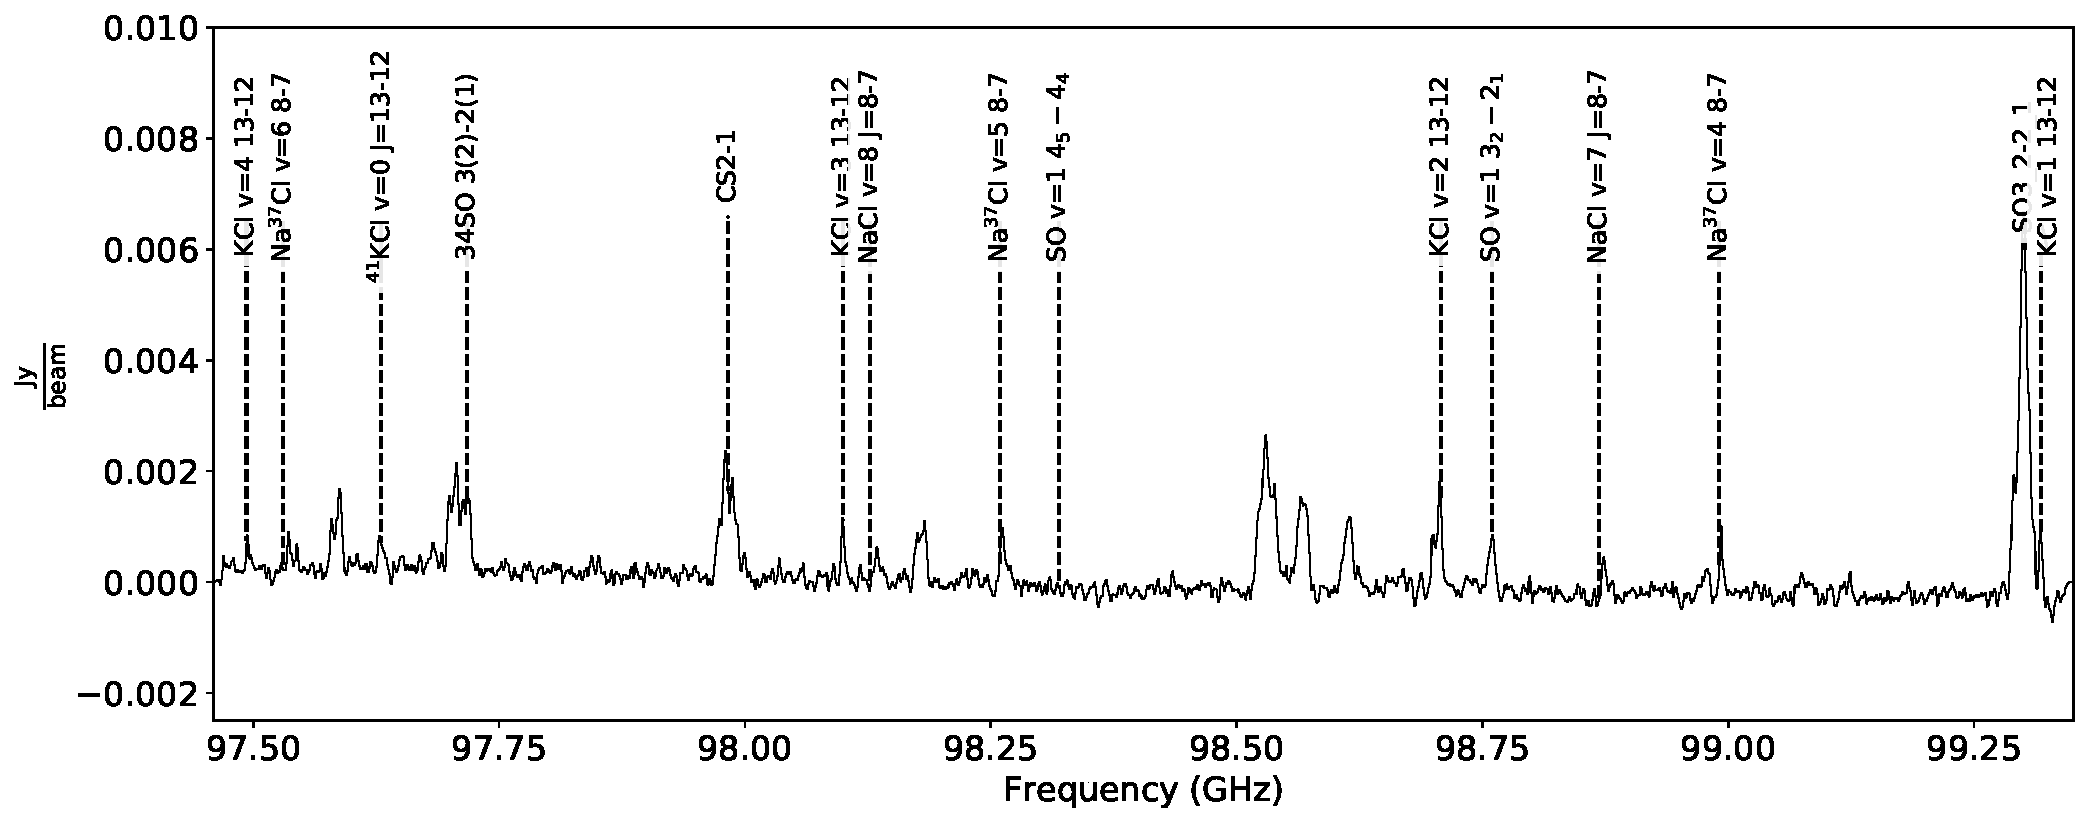
\includegraphics[scale=1,width=6in]{figures/lines_labeled_OrionSourceI_B3_spw2_robust0.5.pdf}
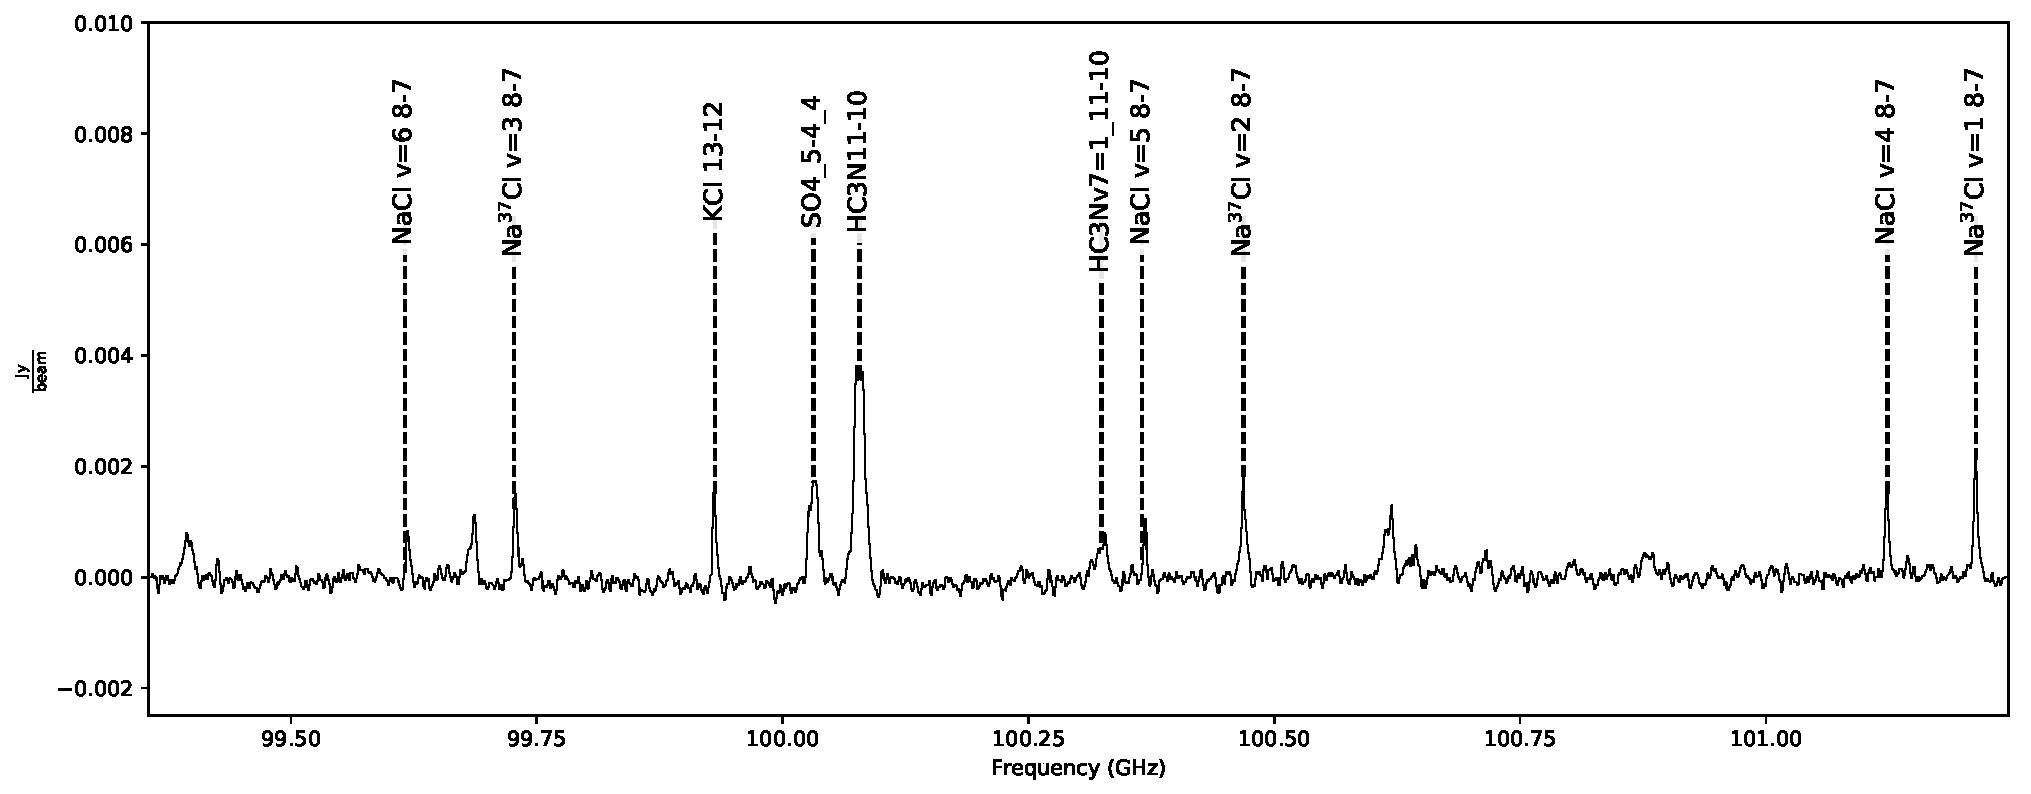
\includegraphics[scale=1,width=6in]{figures/lines_labeled_OrionSourceI_B3_spw3_robust0.5.pdf}
\caption{Stacked spectra  B3}
\label{fig:spectrab3}
\end{figure*}
\begin{figure*}[!htp]
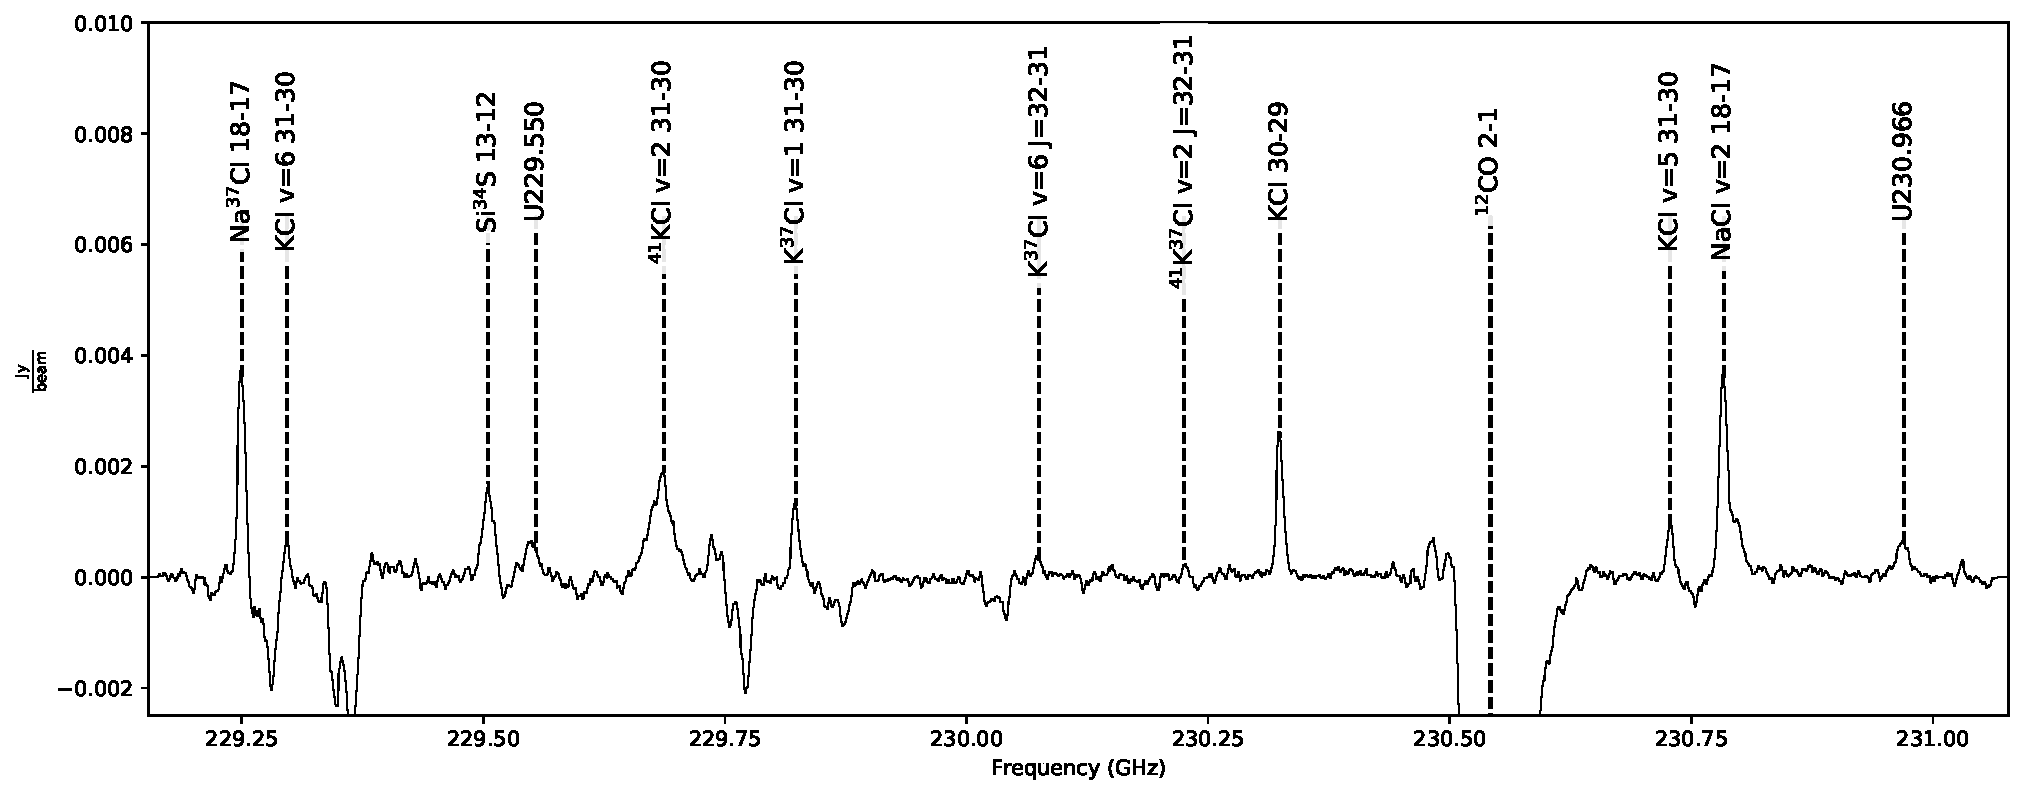
\includegraphics[scale=1,width=6in]{figures/lines_labeled_OrionSourceI_B6_spw0_robust0.5.pdf}
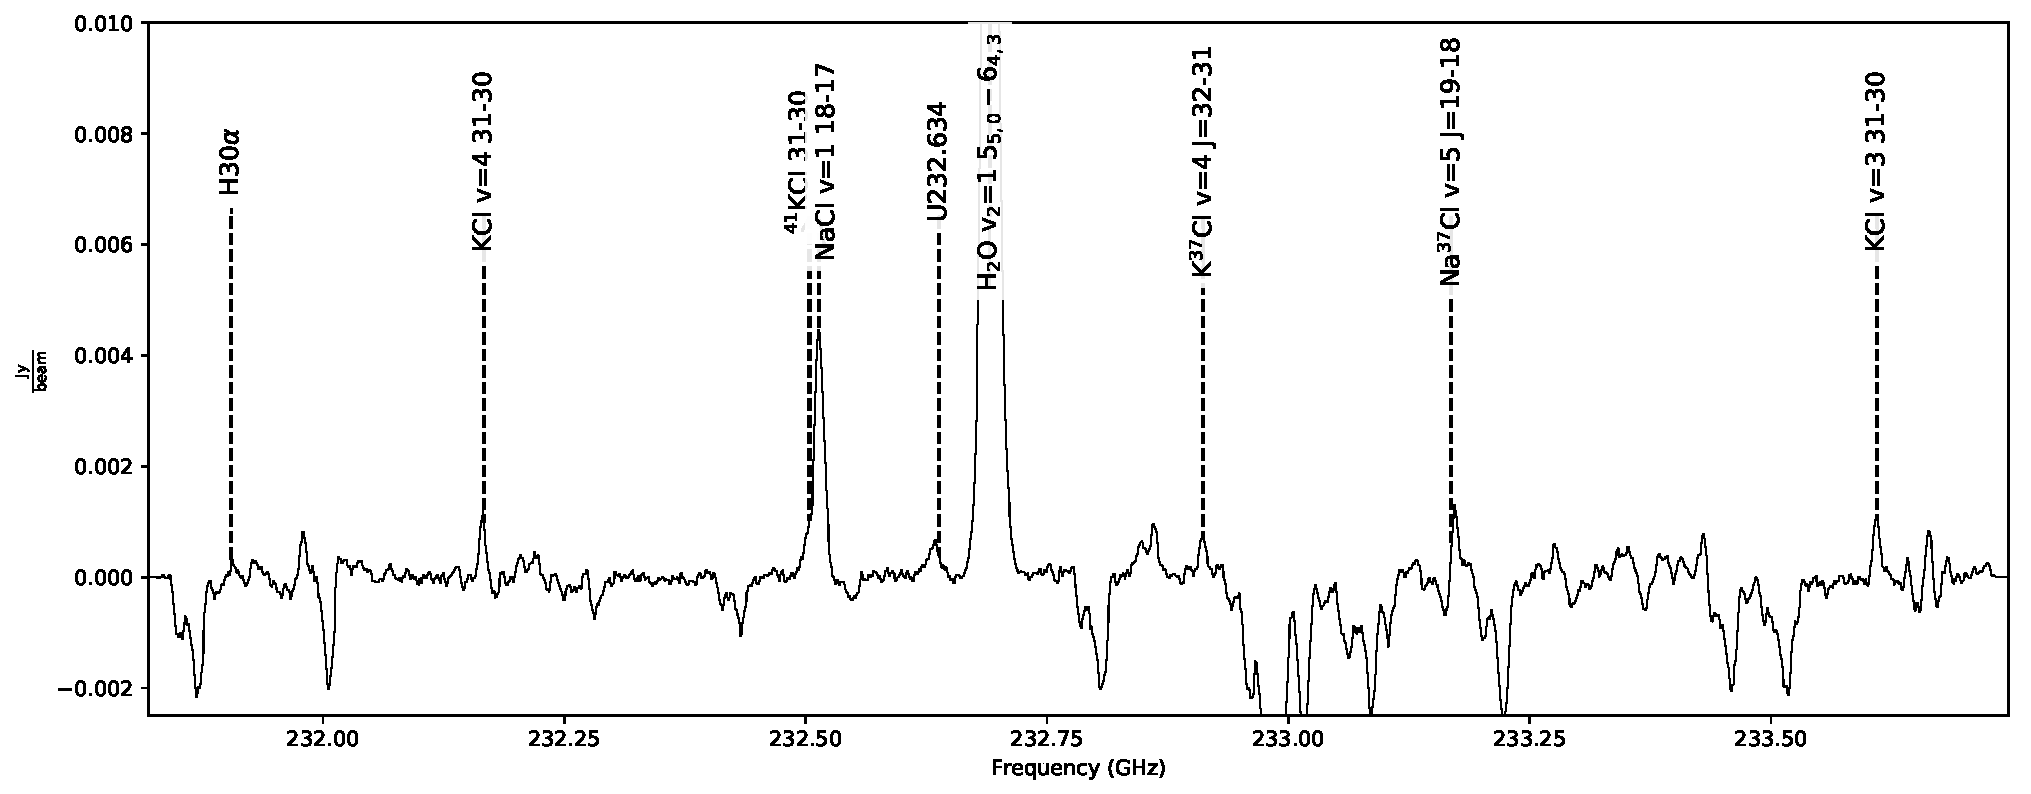
\includegraphics[scale=1,width=6in]{figures/lines_labeled_OrionSourceI_B6_spw1_robust0.5.pdf}
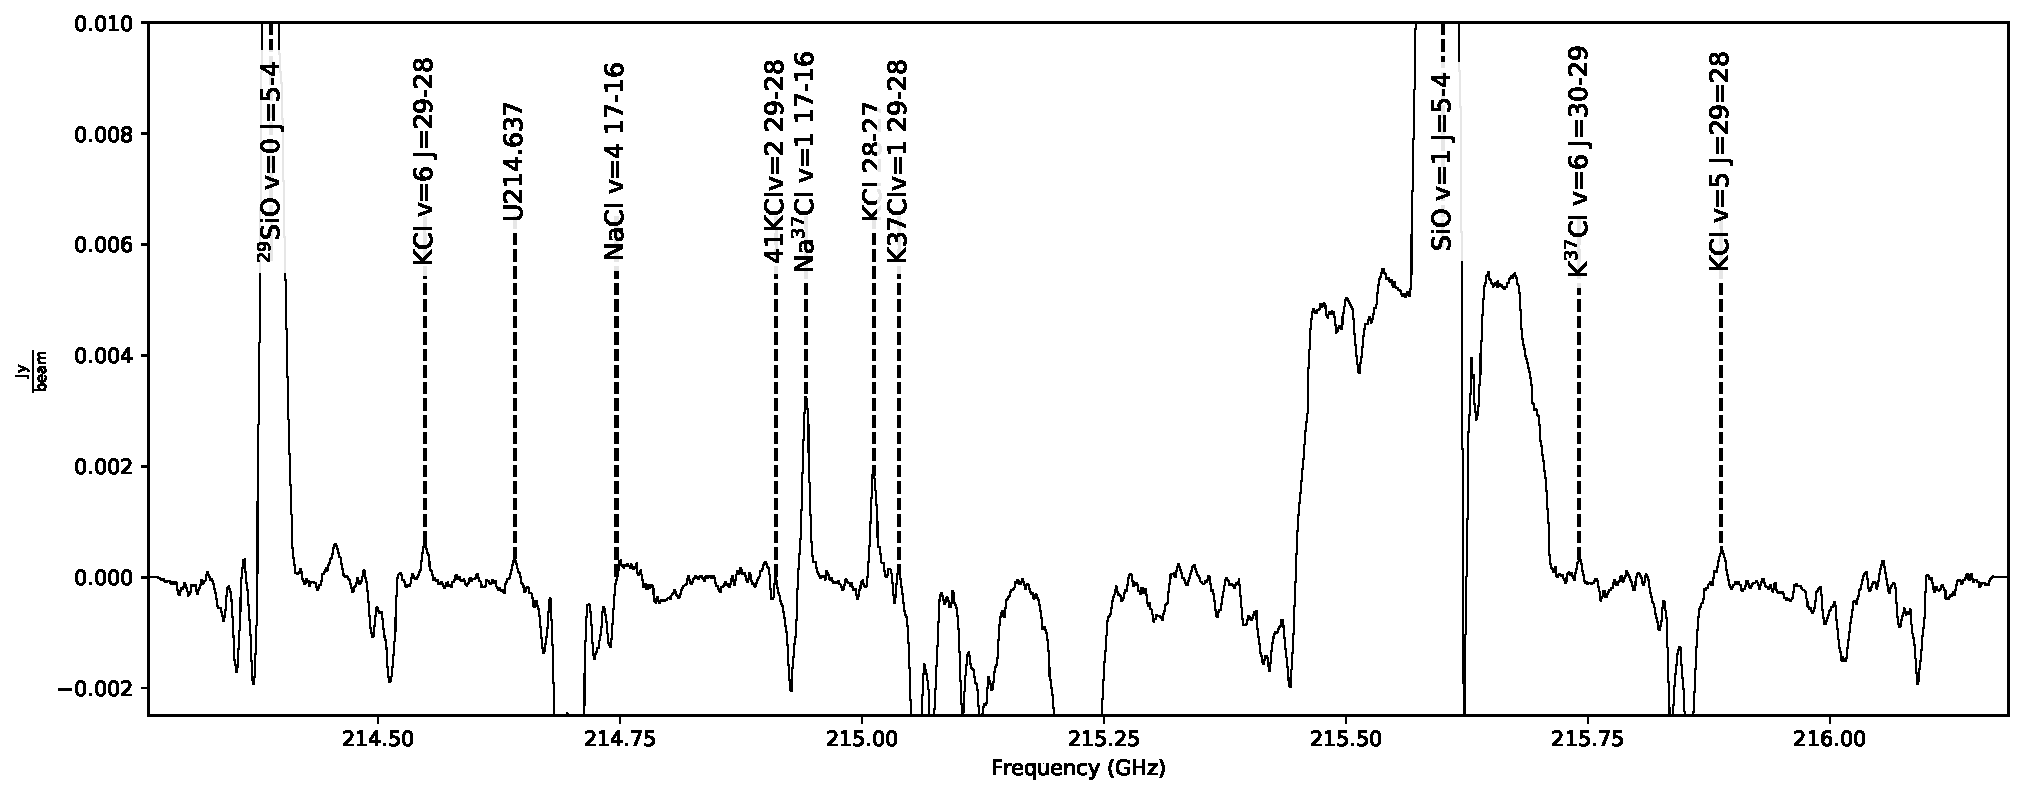
\includegraphics[scale=1,width=6in]{figures/lines_labeled_OrionSourceI_B6_spw2_robust0.5.pdf}
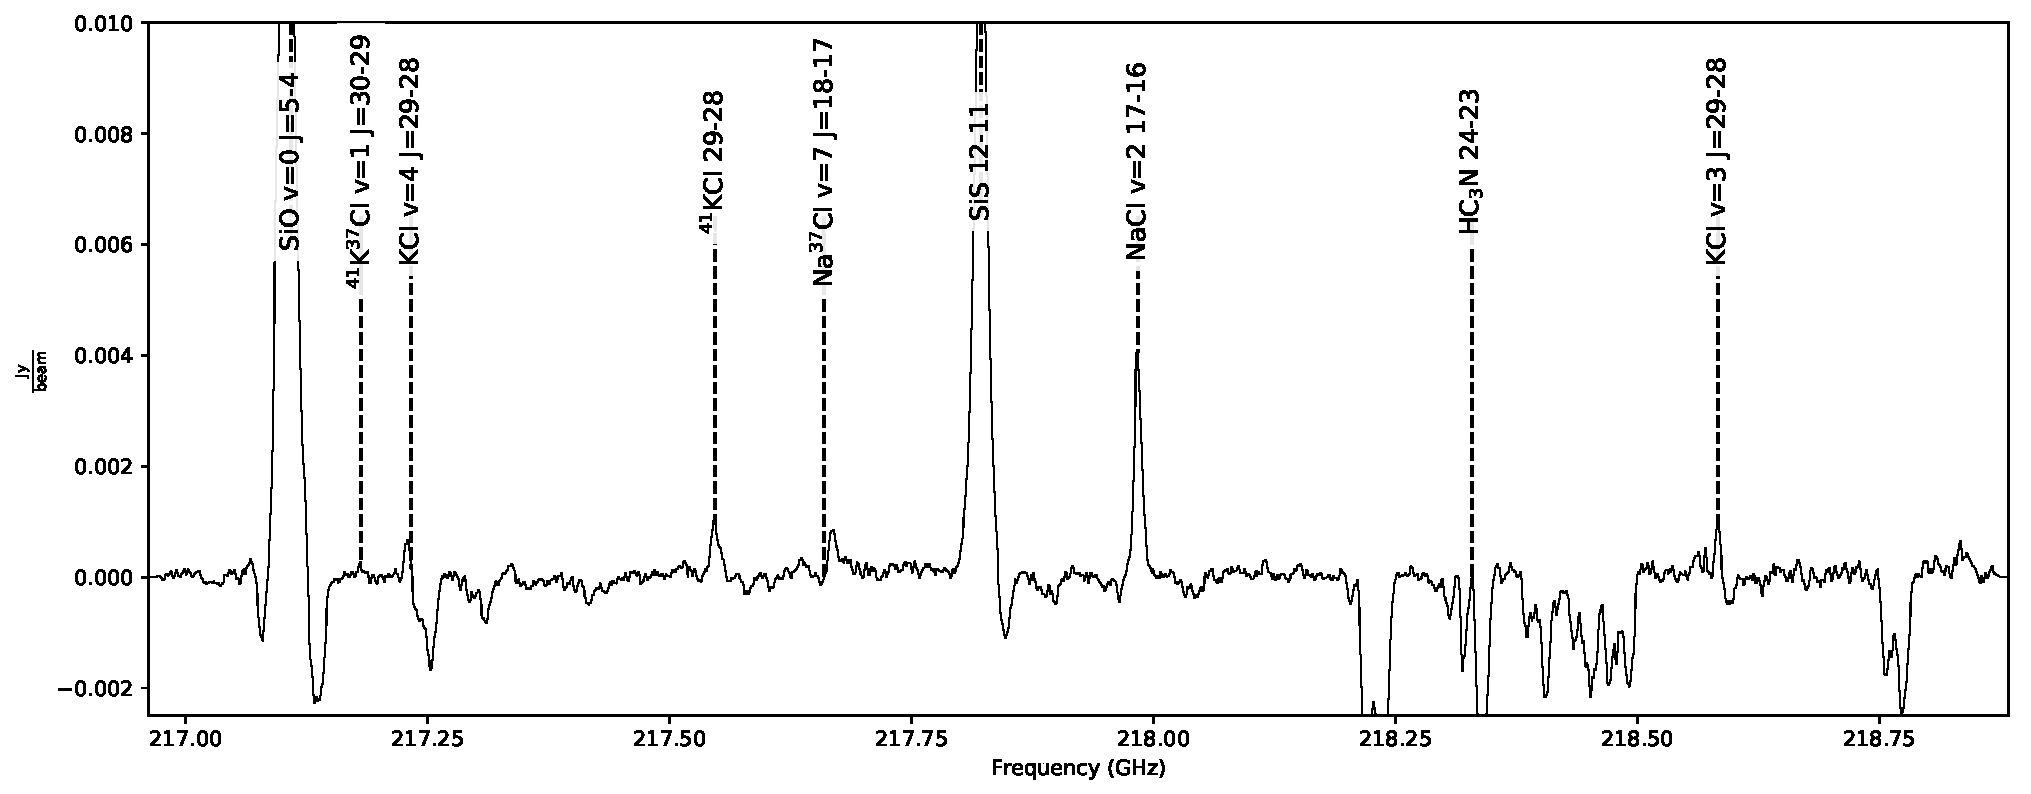
\includegraphics[scale=1,width=6in]{figures/lines_labeled_OrionSourceI_B6_spw3_robust0.5.pdf}
\caption{Stacked spectra B6}
\label{fig:spectrab6}
\end{figure*}
\begin{figure*}[!htp]
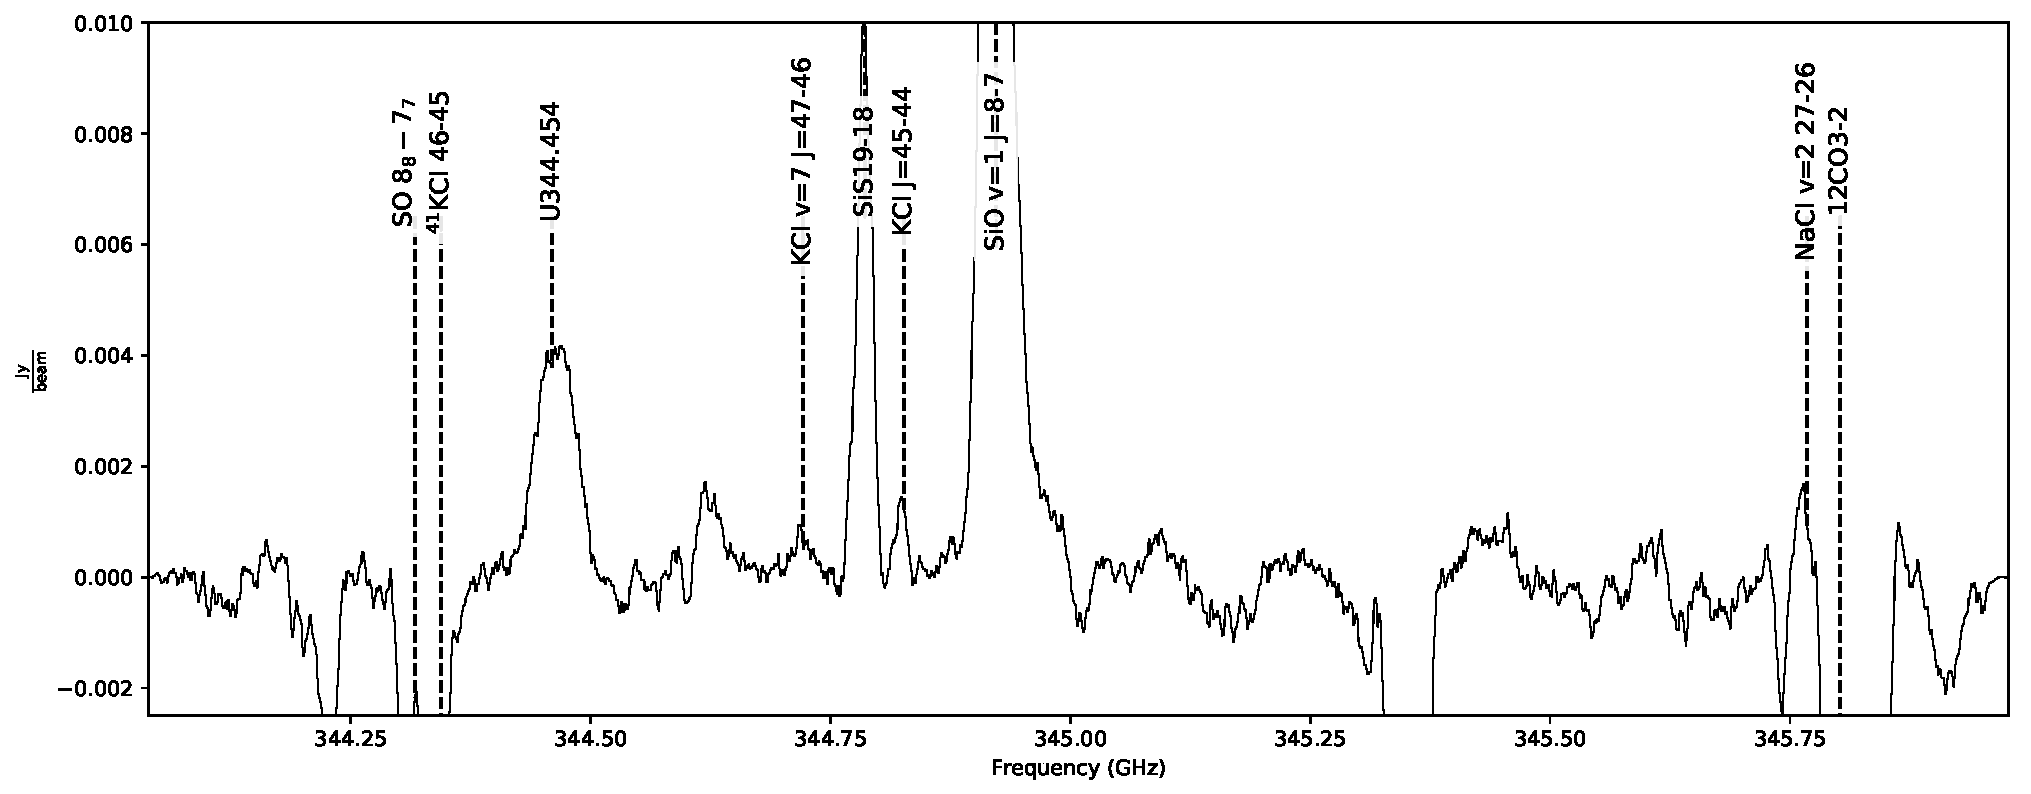
\includegraphics[scale=1,width=6in]{figures/lines_labeled_OrionSourceI_B7.lb_spw0_robust0.5.pdf}
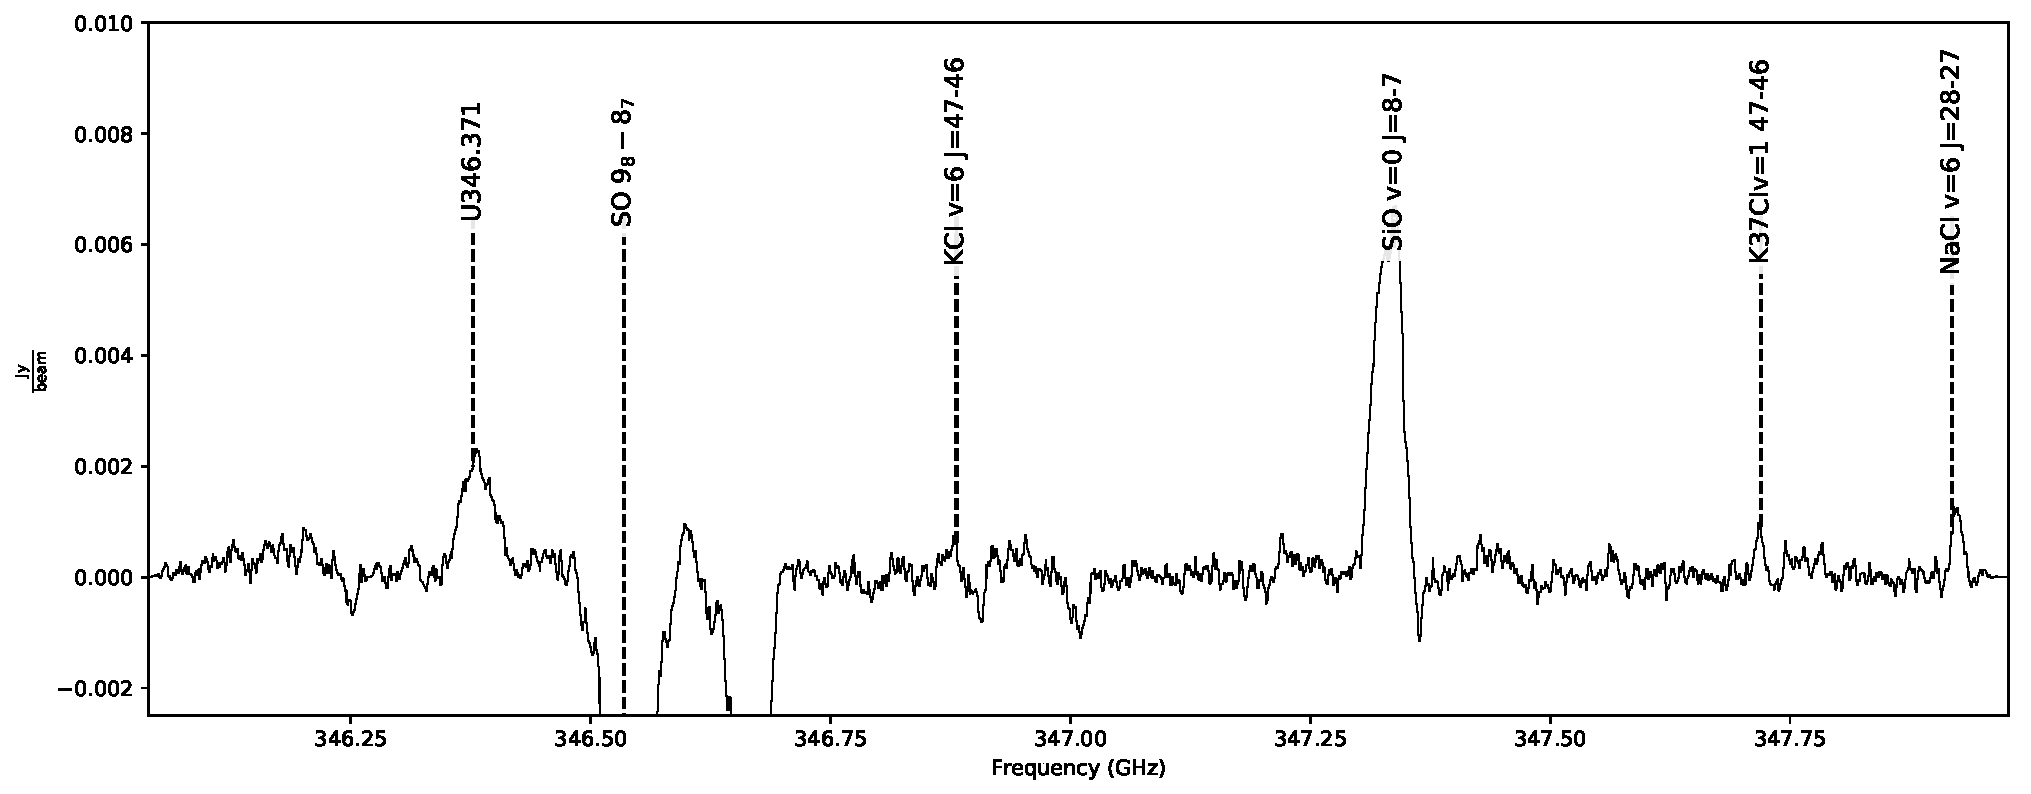
\includegraphics[scale=1,width=6in]{figures/lines_labeled_OrionSourceI_B7.lb_spw1_robust0.5.pdf}
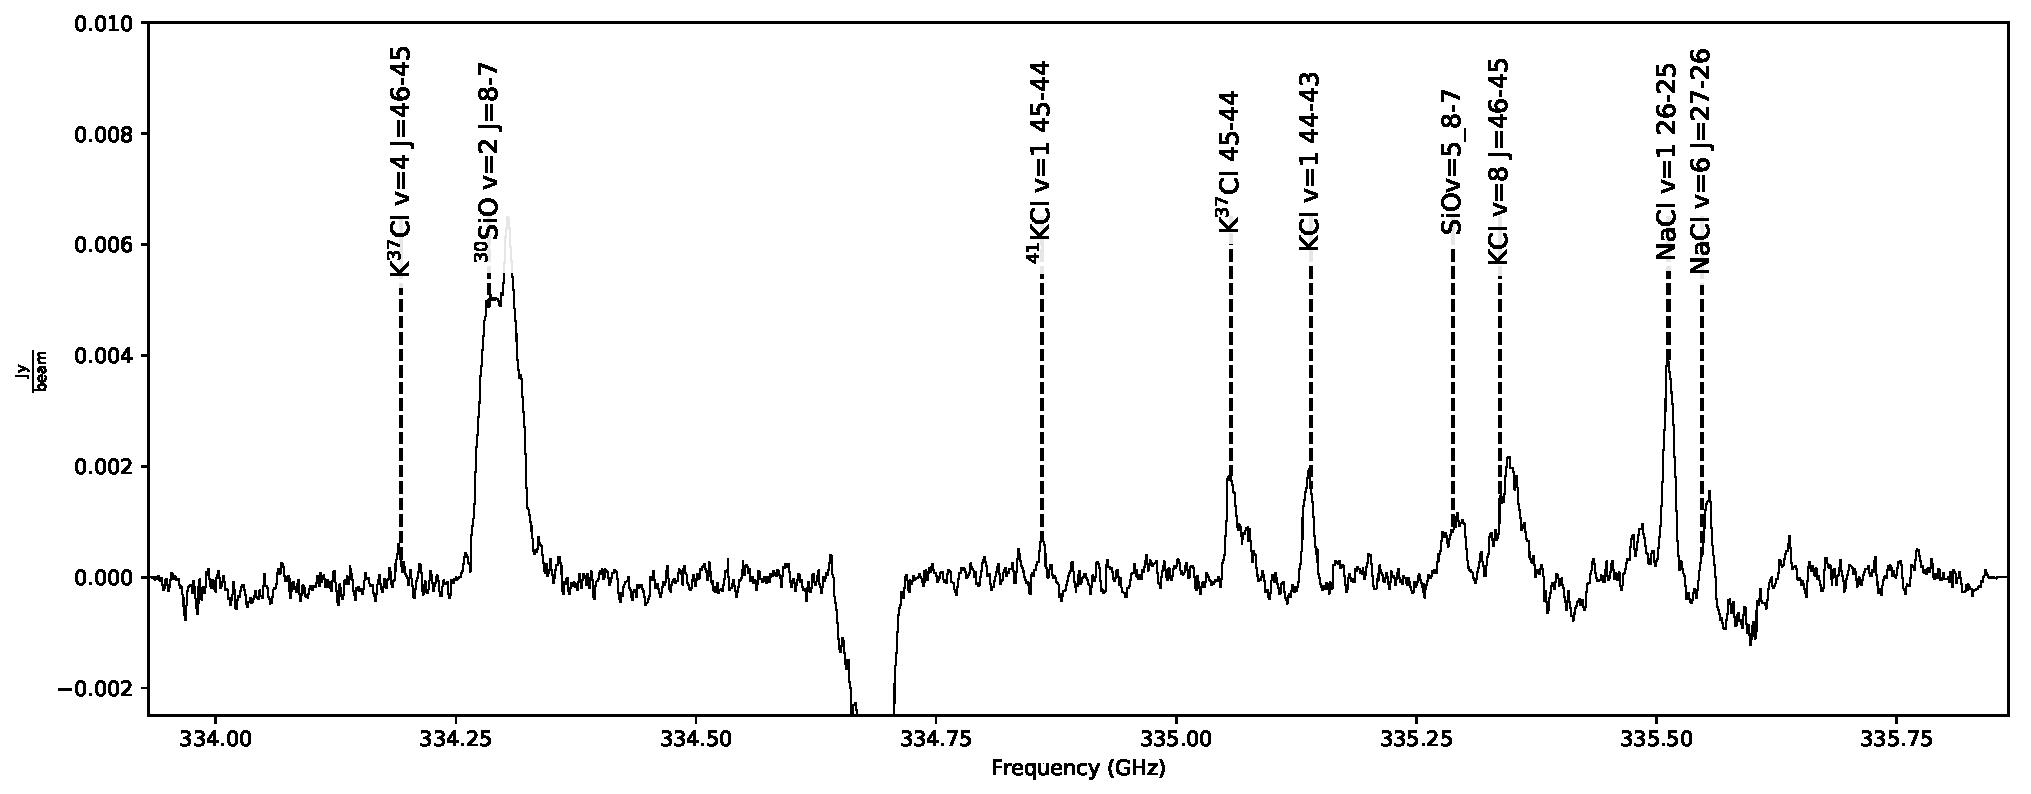
\includegraphics[scale=1,width=6in]{figures/lines_labeled_OrionSourceI_B7.lb_spw2_robust0.5.pdf}
\includegraphics[scale=1,width=6in]{figures/lines_labeled_OrionSourceI_B7.lb_spw3_robust0.5.pdf}
\caption{Stacked spectra B7}
\label{fig:spectrab7}
\end{figure*}

\section{Results}
We have clearly identified the carrier of the majority [what number?]
of unidentified lines in the \citet{Ginsburg2018a} spectra.
The lines have amplitudes in the range 0.5-3 mJy \perbeam, corresponding
to brightness temperatures 5-20 K.

The low observed brightness temperatures suggest that the emission from
these lines is optically thin.


We plot and fit rotational diagrams to measure the abundance and temperature of
these molecules.  However, the results are ambiguous: for each vibrational
state with more than one detected transition, we are able to fit an excitation
temperature, but the abundances of the vibrationally excited states are much
higher than the ground state.  This distribution implies that the lines are
radiatively excited, and suggests that many of the unidentified transitions in
our bandpass may be from uncatalogued higher vibrational states of these same
molecules, since the abundance rises nearly linearly from v=0 to v=4 for NaCl.

The excitation temperatures derived from the rotational diagram fits are in the
range 50-100 K, which implies that the lines are sub-thermally excited.  The
radiation temperature within 50 AU of a $10^4$ \lsun star should be $T_R>500$ K,
so how do we get lower temperatures?
{\color{red} This is a place for some discussion: is it possible that the gas
is cooler and the transitions we're seeing are affected by collisions?
This is the process invoked in \citet{Kaplan2017a}, but it doesn't make sense here:
it requires the gas to be below the radiation temperature.  Also, the critical density
of these transitions is likely to be absurdly high, given their A-values in the 0.1s
range.}

\section{Discussion}
The lines we have reported have only been seen in a small handful of other sources,
all of which were moderately high-mass evolved stars blowing off their envelopes.
The known detections include the carbon star envelope IRC +10216 \citep{Cernicharo1987a},
the post-AGB star envelope CRL 2688 \citep{Highberger2003a}, and the oxygen-rich
evolved star envelopes of VY Canis Majoris and IK Tauri \citep{Milam2007a}.
In these evolved stars, v=0 rotational transitions of NaCl were observed
with rotational temperatures $T_{rot}\sim70-100$ K.
% Carbon star envelope IRC +10216, d ~ 170 pc
% CRL2688 post-AGB * \citep{Highberger2003a} ~ 1 kpc
% IK Tauri, VY Canis Majoris \citep{Milam2007a}

These lines trace a rare physical phenomenon.  They are therefore an excellent tracer
of this phenomenon, assuming they are detected

Sodium and potassium are rarely observed in the dense molecular interstellar medium.
They are usually assumed to be rapidly incorporated into dust grains [cite?  Milam
says this, but there's a better original source].  Since we clearly observe NaCl
and KCl in the atmosphere of the disk, it is clear that there is a zone where either
dust has not yet formed or where dust is destroyed and returned to the gas phase.
{\color{red} What can we say about the dust destruction/sublimation zone?  I need
to do some disk research; there must be a dust sublimation zone at the surfaces
of disks in addition to the radial one.}

\end{document}
